\documentclass[tikz,border=6pt]{standalone}
\usepackage{tikz}
\usetikzlibrary{arrows.meta,positioning,fit}
\definecolor{ink}{HTML}{222222}
\definecolor{inputfill}{HTML}{E8F1FF}
\definecolor{statefill}{HTML}{EAF7EF}
\definecolor{policyfill}{HTML}{FFF4D6}
\definecolor{safetyfill}{HTML}{FDECEC}
\tikzset{
  box/.style={draw=ink, rounded corners=2pt, very thick, align=center, minimum height=8mm, text width=30mm, font=\sffamily\small},
  wide/.style={draw=ink, rounded corners=2pt, very thick, align=left, minimum height=10mm, text width=58mm, font=\sffamily\footnotesize},
  small/.style={draw=ink, rounded corners=2pt, thick, align=center, minimum height=7mm, text width=27mm, font=\sffamily\footnotesize},
  arrow/.style={-{Latex[length=2.2mm]}, very thick, draw=ink}
}
\begin{document}
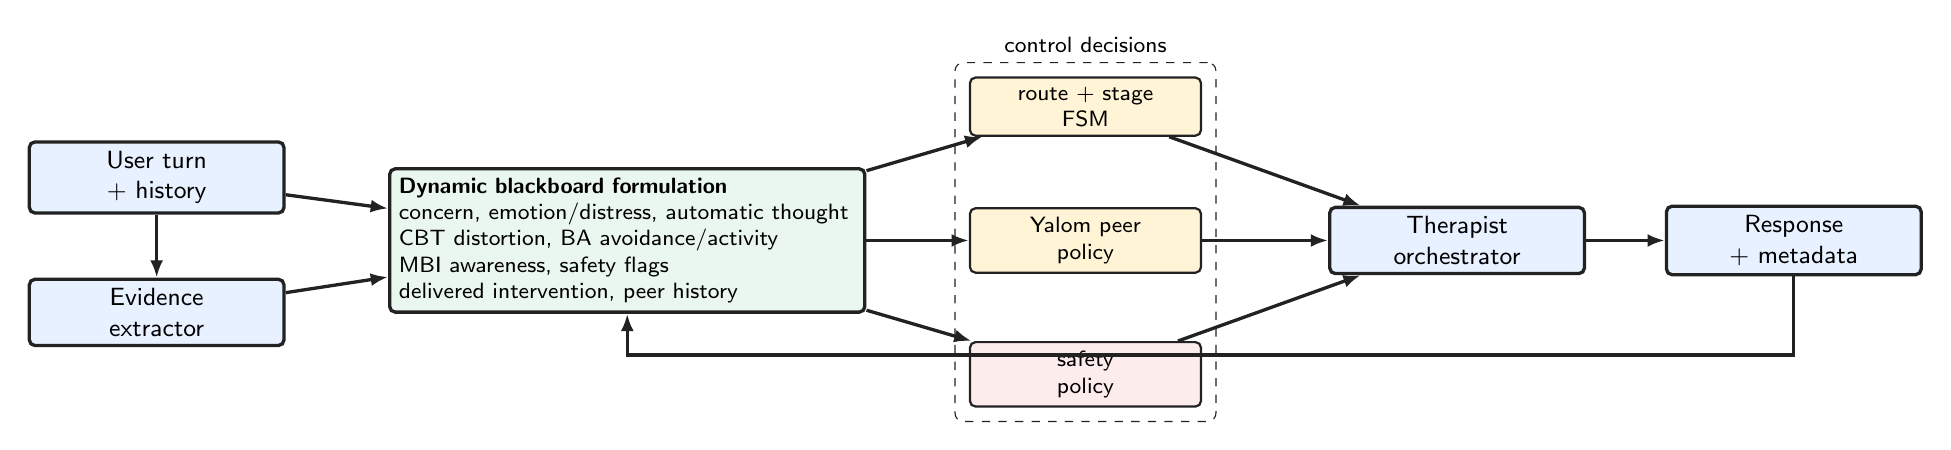
\begin{tikzpicture}[node distance=8mm and 10mm]
  \node[box, fill=inputfill] (turn) {User turn\\+ history};
  \node[box, fill=inputfill, below=of turn] (extractor) {Evidence\\extractor};

  \node[wide, fill=statefill, right=13mm of turn, yshift=-8mm] (formulation) {
    \textbf{Dynamic blackboard formulation}\\
    concern, emotion/distress, automatic thought\\
    CBT distortion, BA avoidance/activity\\
    MBI awareness, safety flags\\
    delivered intervention, peer history
  };

  \node[small, fill=policyfill, right=13mm of formulation, yshift=17mm] (route) {route + stage\\FSM};
  \node[small, fill=policyfill, right=13mm of formulation] (peer) {Yalom peer\\policy};
  \node[small, fill=safetyfill, right=13mm of formulation, yshift=-17mm] (safety) {safety\\policy};

  \node[box, fill=inputfill, right=16mm of peer] (orchestrator) {Therapist\\orchestrator};
  \node[box, fill=inputfill, right=of orchestrator] (log) {Response\\+ metadata};

  \draw[arrow] (turn) -- (extractor);
  \draw[arrow] (turn) -- (formulation);
  \draw[arrow] (extractor) -- (formulation);
  \draw[arrow] (formulation) -- (route);
  \draw[arrow] (formulation) -- (peer);
  \draw[arrow] (formulation) -- (safety);
  \draw[arrow] (route) -- (orchestrator);
  \draw[arrow] (peer) -- (orchestrator);
  \draw[arrow] (safety) -- (orchestrator);
  \draw[arrow] (orchestrator) -- (log);
  \draw[arrow] (log.south) |- ++(0,-10mm) -| (formulation.south);

  \node[draw=ink, rounded corners=3pt, dashed, fit=(route)(peer)(safety), inner sep=5pt, label={[font=\sffamily\footnotesize]above:control decisions}] {};
\end{tikzpicture}
\end{document}
